\documentclass{hw-template}
\title{MA587 HW 3}
\author{Kyle Hansen}
\date{31 March 2026}

\usepackage{cancel}

\newcommand{\p}{^\prime}
\newcommand{\pr}{\prime}
\newcommand{\intI}{\int\limits_{I}}
\newcommand{\intOm}{\int_{\Omega}}
\newcommand{\hlin}{{H_0^1}}
\newcommand{\hOne}{{H^1}}
\newcommand{\ltwo}{{L^2}}
\newcommand{\htwo}{{H^2}}
\newcommand{\hz}{{H^2_0}}


\begin{document}
\maketitle

\section{Second order Problem}

\subsection{}

First, the differential equation is multiplied by test vector $v \in V$ and integrated over the domain,

\begin{equation}
    -\int_{0}^1 u^{\pr\pr}v dx = \int_{0}^1 f v dx
\end{equation}

Gauss Divergence theorem is used to reduce the left-hand side,

\begin{equation}
    - \left[ \cancelto{_{v(0) = v(1) = 0}}{u'v \Big|_{0}^1} - \int_{0}^1 u\p v\p dx \right]= \int_{0}^1 f v dx
\end{equation}

which yields the final weak form,

\begin{align}
    a(u, v) &= L(v)\; \forall v \in V\\
    a(u, v) &= \int_{0}^1 u\p v\p dx\\
    L(v) &= \int_{0}^1 f v dx
\end{align}

\subsection{}

To show that $a$ is symmetric, note that the multiplication inside the integral is commutative, so

\begin{equation}
    a(u, v) = \int_{0}^1 u\p v\p dx = \int_{0}^1 v\p u\p dx = a(v, u)
\end{equation}

and thus $a$ is symmetric. To show that $a$ is continuous, first note that

\begin{align}
    \norm{u}_{\hlin}^2 &= \norm{u}_{\ltwo}^2 + \norm{u\p}_{\ltwo}^2\\
    \norm{u\p}_{\ltwo}^2 &\leq \norm{u}_{\hlin}^2\\
    \norm{u\p}_{\ltwo} &\leq \norm{u}_{\hlin}\label{eq:p1-lemma}
\end{align}

and also

\begin{equation}
    \norm{u}_{\ltwo} \leq \norm{u}_{\hlin}.\label{eq:p1-lemma2}
\end{equation}

By the Cauchy-Schwarz (CS) inequality, 

\begin{equation}
    \int_0^1 u\p v\p dx = \ip{u\p}{v\p}_{\ltwo} \leq \norm{u\p}_{\ltwo} \norm{v\p}_{\ltwo},
\end{equation}

and thus, using \autoref{eq:p1-lemma}, \

\begin{equation}
    \int_0^1 u\p v\p dx \leq \norm{u}_{\hlin} \norm{v}_{\hlin},
\end{equation}

and $a$ is continuous. To show $L(v)$ is continuous, apply the CS inequality,

\begin{equation}
    \int_0^1 fv dx = \ip{f}{v}_{\ltwo} \leq \norm{f}_\ltwo \norm{v}_\ltwo
\end{equation}

and apply \autoref{eq:p1-lemma2},

\begin{equation}
    \int_0^1 fv dx \leq \norm{f}_\ltwo \norm{v}_\hlin.
\end{equation}


\subsection{}

To show that $a$ is coercive, consider that

\begin{align}
    |v(x)| &= \left|\cancel{v(0)} + \int_0^x v\p (s) ds \right|\\
    |v(x)| &\leq \int_0^1 |v\p (s)| ds = \ip{1}{v\p}_\ltwo.
\end{align}

Then, using the CS inequality,

\begin{align}
    |v(x)| &\leq \norm{1}_\ltwo \norm{v\p}_\ltwo\\
    \norm{v(x)}_\ltwo &\leq \norm{(\norm{v\p}_\ltwo)}_\ltwo\\
    \norm{v(x)}_\ltwo &\leq \norm{v\p}_\ltwo
\end{align}

\subsection{}

\textbf{AI use note}: To complete the coding portion of this assignment, I did not use AI to obtain the solution, instead modifying FEniCS' own demo problems. The code for this problem was based on \href{{https://github.com/FEniCS/dolfinx/blob/main/python/demo/demo_poisson.py}}{demo\_poisson.py}. Gemini \textit{was} used to aid in plotting solutions for all three problems.

Some numerical results are displayed in \autoref{fig:p1-results}, with $L_2$ and $L_\infty$ error listed in \autoref{tab:p1-results}. Here, the results are within double-precision roundoff error when degree-2 polynomials are used in each cell, since the exact solution is a quadratic polynomial, and thus the finite element method calculates the exact solution, even with only one cell. When using degree-1 polynomials in each cell, the error quickly converges (approximately linearly) when more cells are used.

\begin{figure}[h]
    \centering
    \begin{subfigure}{0.45\linewidth}
        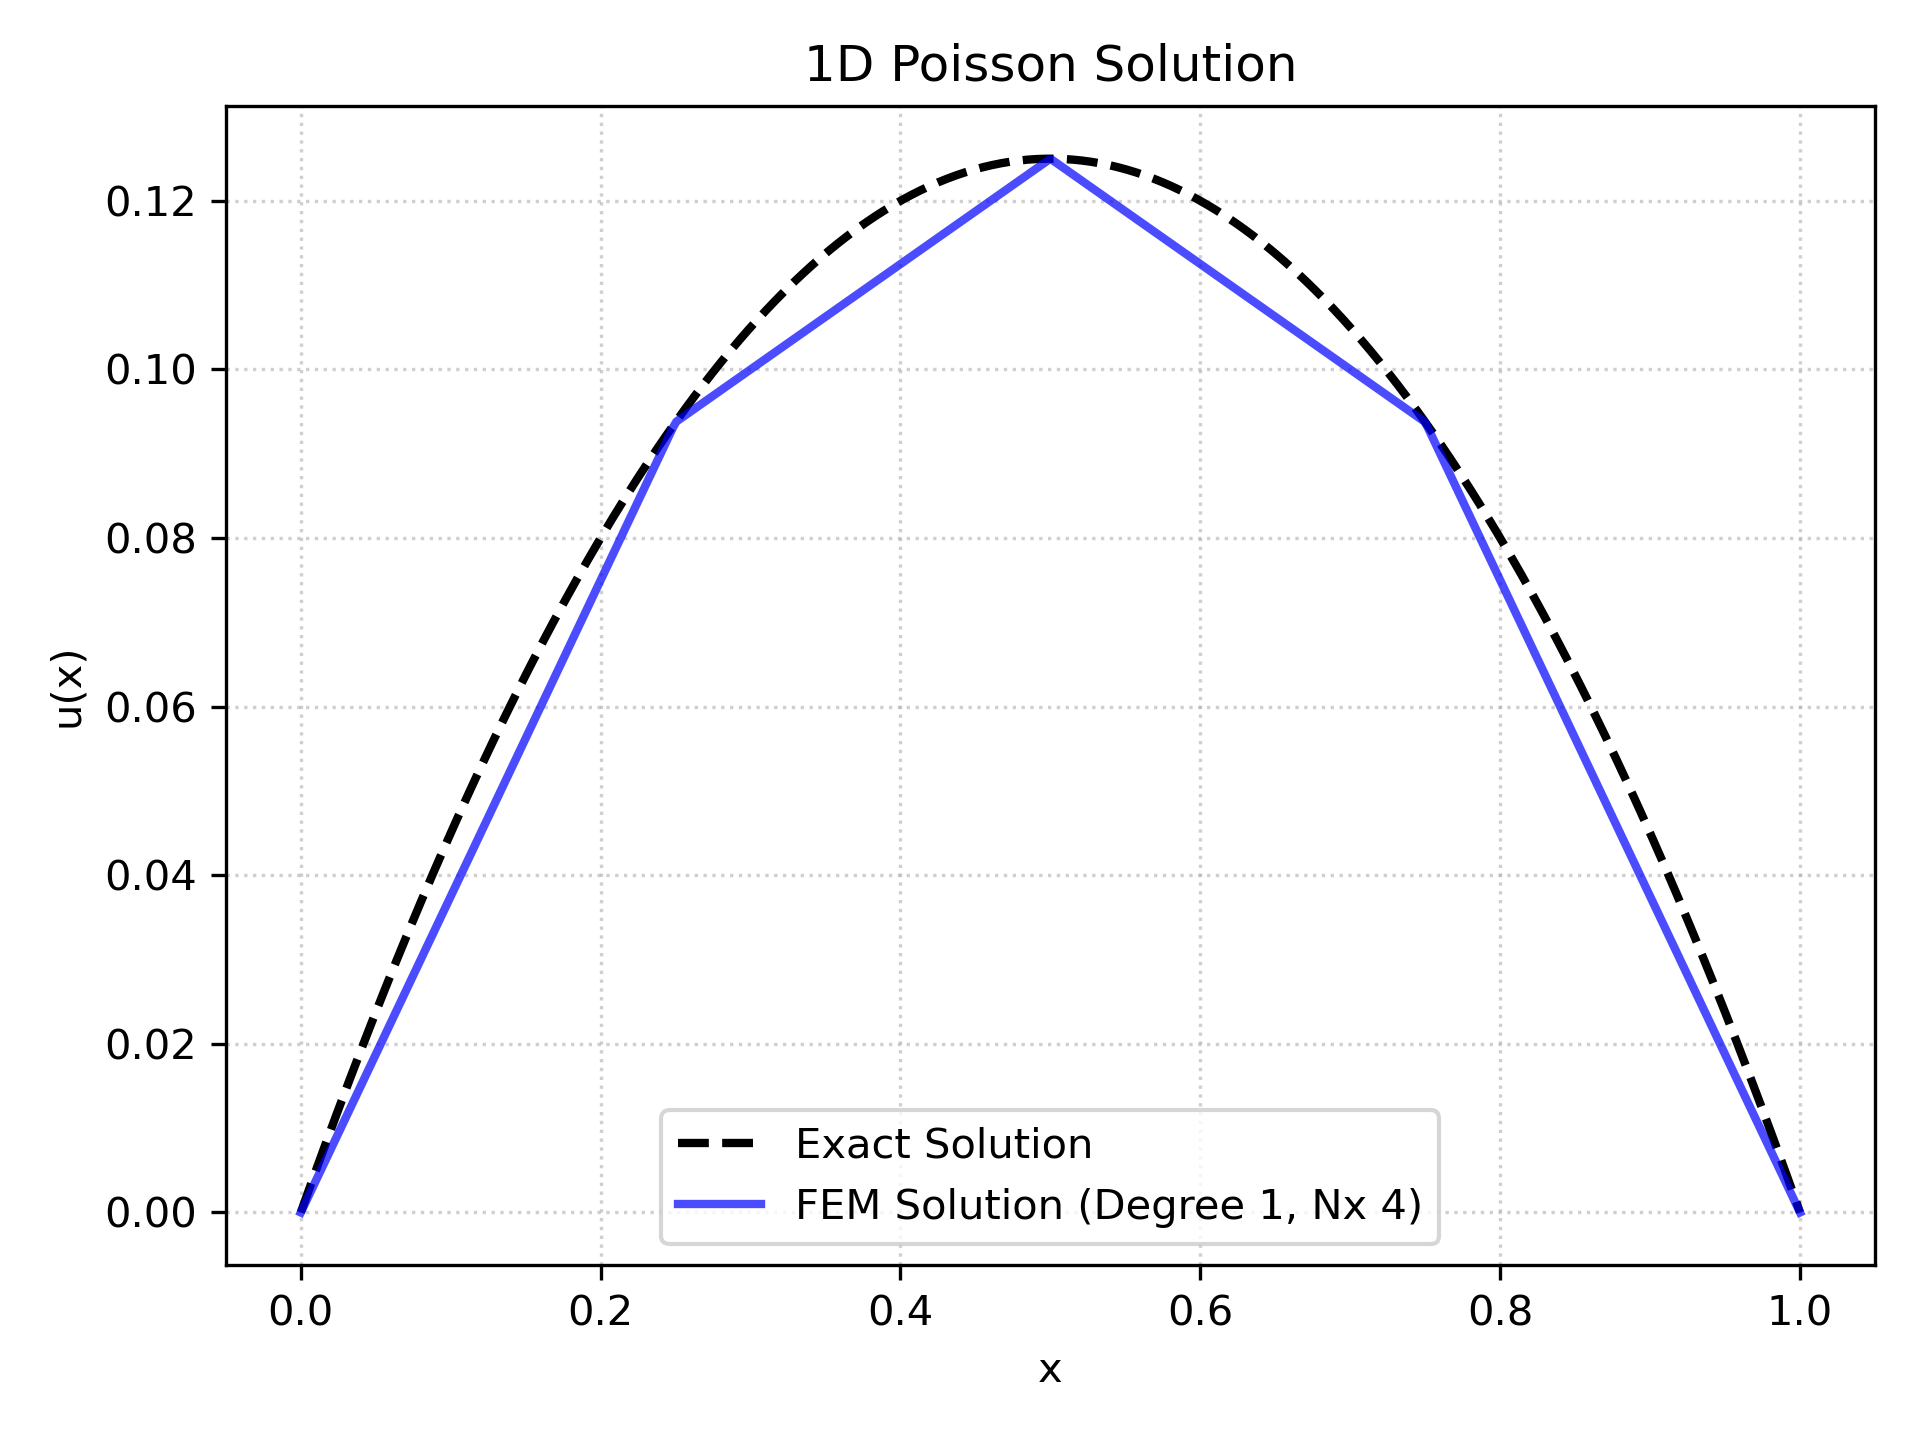
\includegraphics[width=\linewidth]{out_poisson/prob1_n4_d1.png}
        \caption{$P^1$, 4 cells}
    \end{subfigure}
    \begin{subfigure}{0.45\linewidth}
        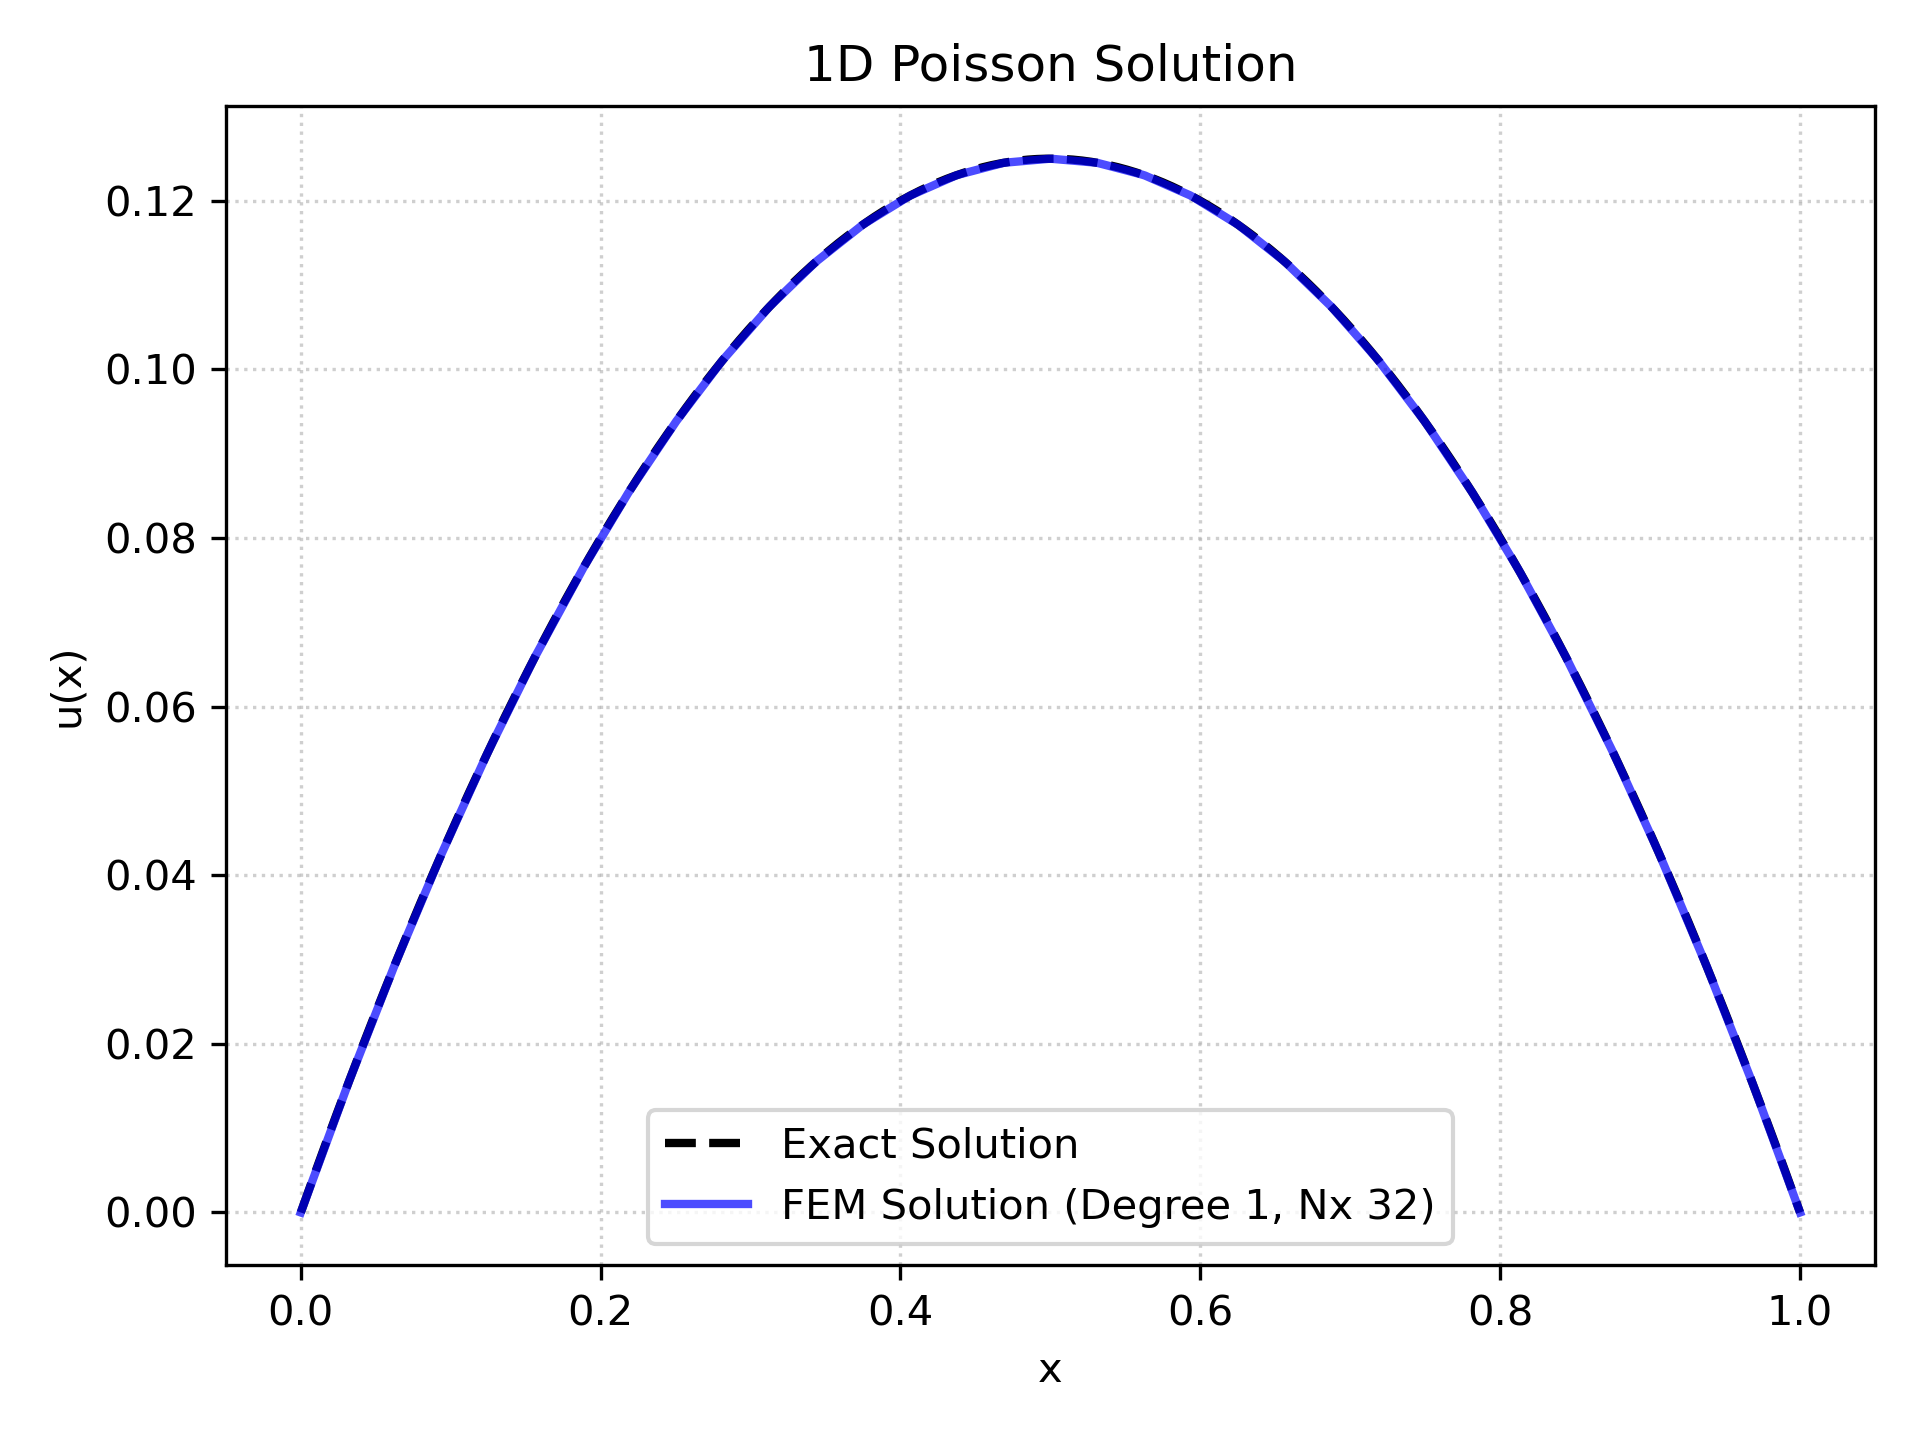
\includegraphics[width=\linewidth]{out_poisson/prob1_n32_d1.png}
        \caption{$P^1$, 32 cells}
    \end{subfigure}

    \begin{subfigure}{0.45\linewidth}
        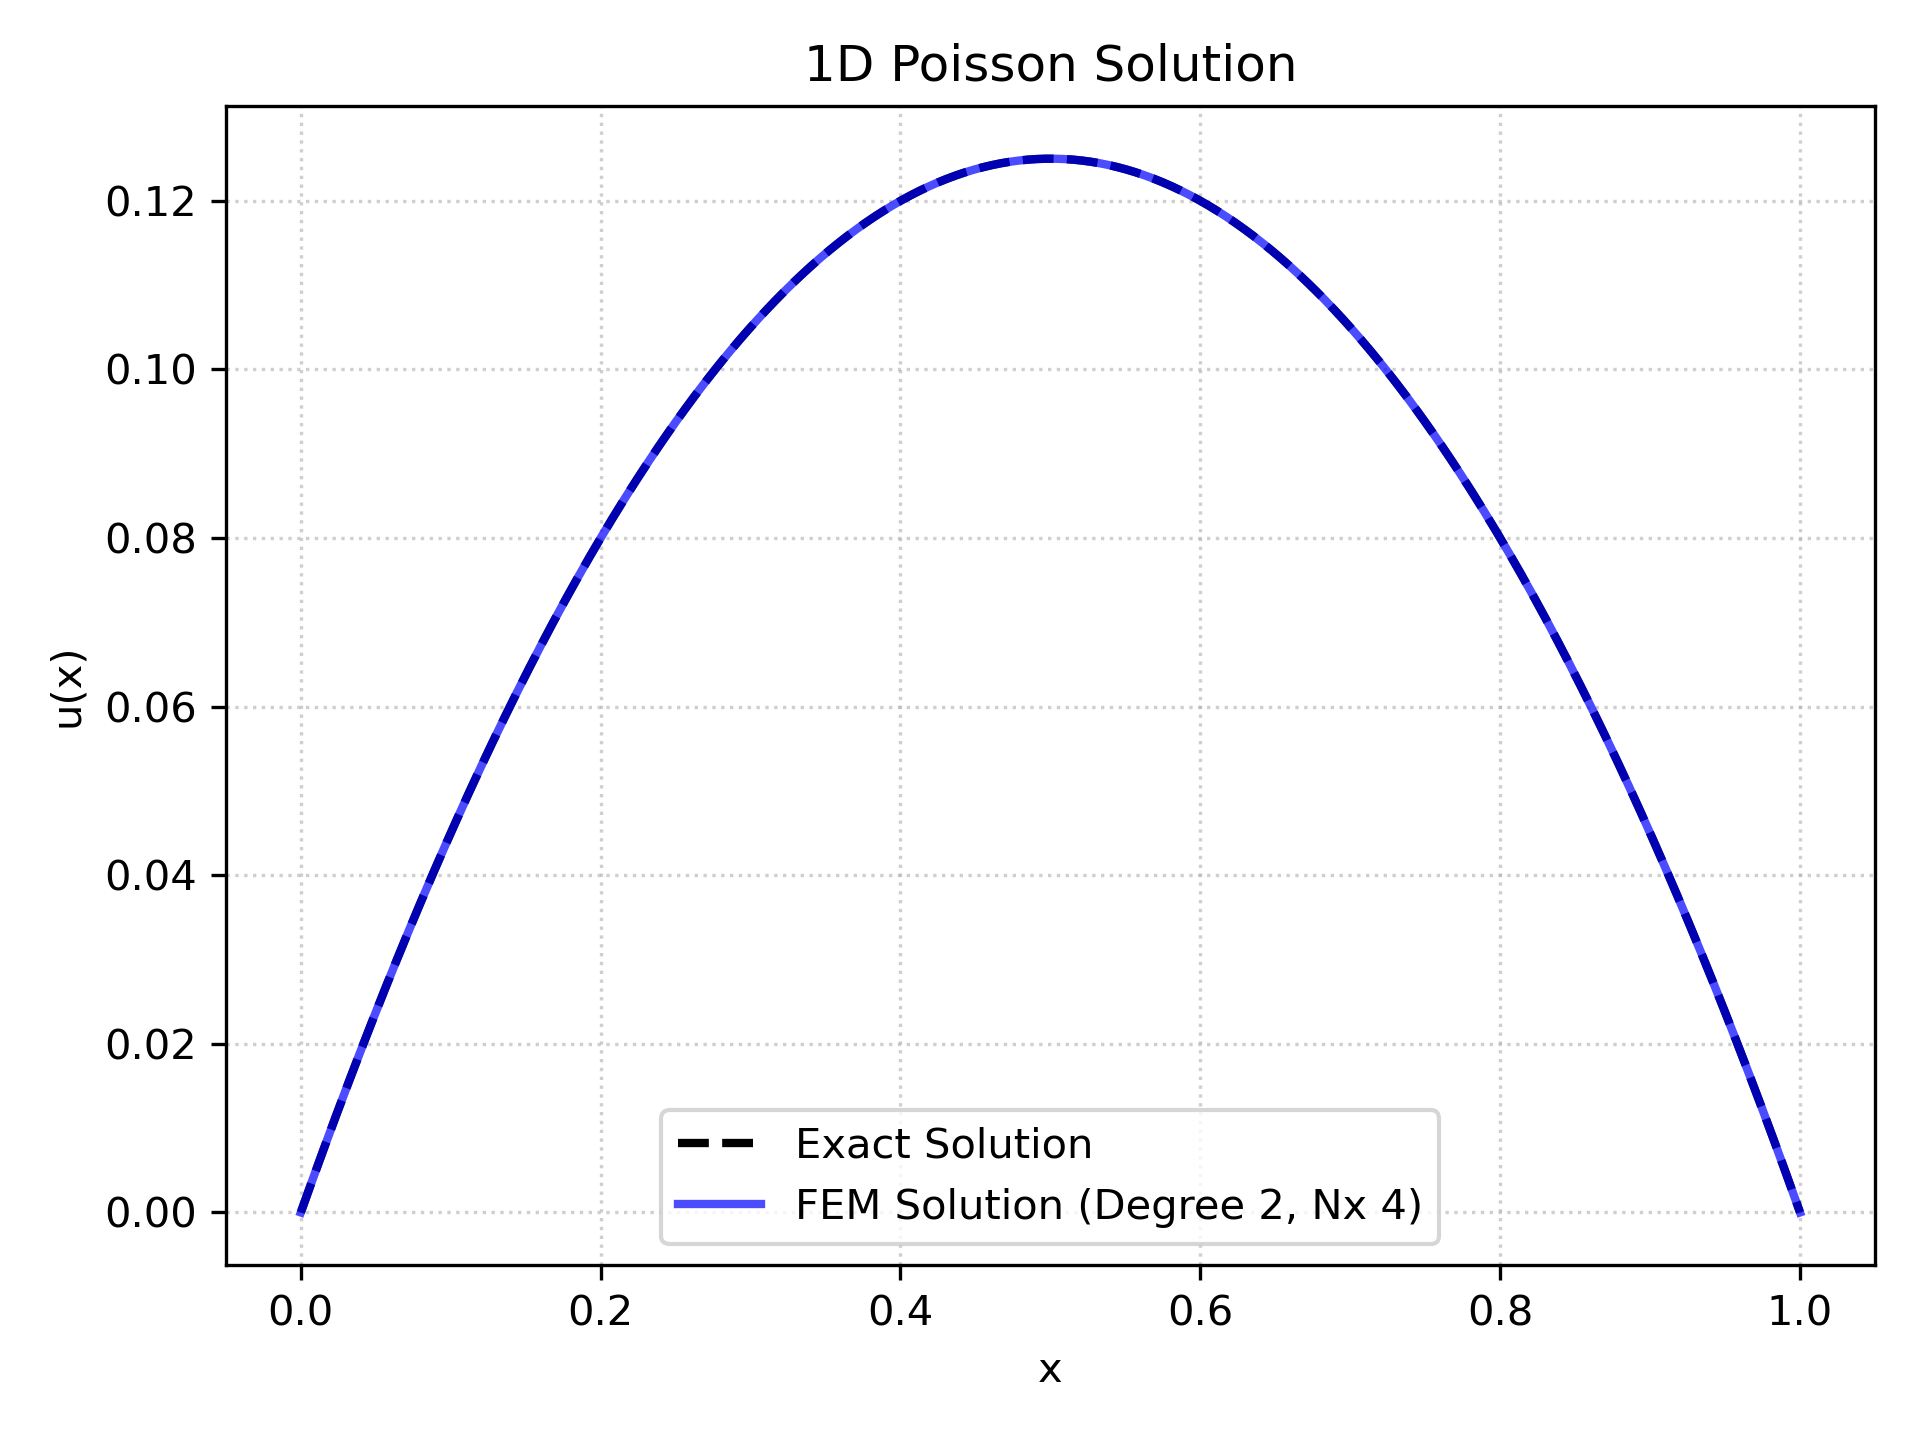
\includegraphics[width=\linewidth]{out_poisson/prob1_n4_d2.png}
        \caption{$P^2$, 4 cells}
    \end{subfigure}

    \caption{1D Poisson Results}\label{fig:p1-results}
\end{figure}

\begin{table}[h]
    \caption{1D Poisson Results}\label{tab:p1-results}

    \centering
    \begin{tabular}{c|c|c}
        $N_x, P^1$ & L2 error & Max. pointwise error\\
        4& 5.705e-03 & 7.812e-03\\
        8& 1.863e-03 & 2.551e-03\\
        16& 3.566e-04 & 4.883e-04\\
        32  & 8.915e-05 & 1.221e-04 
    \end{tabular}
    \begin{tabular}{c|c|c}
        $N_x, P^2$ & L2 error & Max. pointwise error\\
        4&    8.037e-17 & 1.388e-16\\
        8&    1.175e-16 & 1.804e-16\\
        16&   1.267e-15 & 1.818e-15\\
        32  & 5.075e-15 & 7.175e-15 
    \end{tabular}
\end{table}

% TODO fenicxs problem

\section{Poincare Inequality}

\subsection{}

Similarly to the previous problem, and using the notation $x_1 = x, x_2 =$

\begin{align}
    v(x, y) &= \cancel{v(0, y)} + \int_0^x \frac{\partial v(s, y)}{\partial x} ds\\
    v(x, y)^2 &= \left(\int_0^x \frac{\partial v(s, y)}{\partial x} ds \right)^2.
\end{align}

Then, by the CS inequality,

\begin{equation}
    v(x, y)^2 \leq \int_0^x \left({\frac{\partial v(s, y)}{\partial x}}\right)^2 ds.
\end{equation}

Since the term inside the integral is strictly non-negative, 

\begin{equation}
    v(x, y)^2 \leq \int_0^1 \left({\frac{\partial v(s, y)}{\partial x}}\right)^2 ds.
\end{equation}

Then, since $\norm{\nabla v}^2 = \left(\frac{\partial v}{\partial x} \right)^2 + \left(\frac{\partial v}{\partial y} \right)^2$ and thus $\frac{\partial v}{\partial x}^2 \leq \norm{\nabla v}^2$,

\begin{equation}
    v(x, y)^2 \leq \int_0^1  \norm{\nabla v}^2   dx.
\end{equation}

Integrating this once more over the domain,

\begin{equation}
    \int_0^1 v(x, y)^2 \leq \int_0^1\int_0^1  \norm{\nabla v}^2   dx dx
\end{equation}

\begin{equation}
    \int_0^1 v(x, y)^2 \leq \int_0^1  \norm{\nabla v}^2   dx.
\end{equation}

\subsection{}

Note that $\norm{v}_\htwo^2 = \norm{v}_\ltwo^2 + \norm{\nabla v}_\ltwo^2 + \norm{\Delta v}_\ltwo^2$. Begining with the $\norm{v}_\ltwo^2$ term, as in the previous part,

\begin{align}
    v(x, y) &= \cancel{v_x(0, y)} + \int_0^x v_x(s, y)ds\\
    v(x, y)^2 &=\left(\int_0^x v_x(s, y)ds\right)^2\label{eq:x-only}.
\end{align}

Similarly,

\begin{equation}
    v_x(s, y) = \cancel{v_x(x, 0)} + \int_0^y v_{xy}(s,q)dq,
\end{equation}

so, plugging this into \autoref{eq:x-only},

\begin{equation}
    v(x, y)^2 = \left(\int_0^x \int_0^y v_{xy}(s,q)ds \, dq \right)^2
\end{equation}

Applying the CS inequality twice,

\begin{equation}
    v(x, y)^2 \leq \int_0^x \int_0^y v_{xy}(s,q)^2 ds \, dq.
\end{equation}

Since the term inside the integral is strictly non-negative,

\begin{equation}
    v(x, y)^2 \leq \int_0^\Gamma \int_0^\Gamma v_{xy}(x, y)^2 dx \, dy.
\end{equation}

where $\Gamma$ is the length of the square. Applying Green's formula and using the boundary conditions,

\begin{equation}
    v(x, y)^2 \leq \intOm v_{xx}v_{yy}d\mu \leq \intOm |v_{xx}||v_{yy}|d\mu.
\end{equation}

Since 

\begin{equation}
    |\Delta v|^2 = |v_{xx}|^2 + 2 |v_{xx}| |v_{yy}| + |v_{yy}|^2,\label{eq:expansion}
\end{equation}

and thus $|v_{xx}| |v_{yy}| \leq \frac{1}{2}|\Delta v|^2$,

\begin{equation}
    v(x, y)^2 \leq \frac{1}{2} \intOm |\Delta v|^2 d\mu.
\end{equation}

Integrating over the domain yields

\begin{equation}
    \intOm v(x, y)^2 d \mu \leq \frac{1}{2} \Gamma^2\intOm |\Delta v|^2 d\mu,\label{eq:first-inequality}
\end{equation}

where again $\Gamma$ is the length of the square. Next, to show the inequality for $\norm{\nabla v}_\ltwo^2$, again apply the expansion in \autoref{eq:expansion},

\begin{equation}
   |\nabla v|^2 = |v_{xx}|^2 + |v_{yy}|^2 \leq |\Delta v|^2,
\end{equation}

then integrate over the domain to yield

\begin{equation}
    \intOm |\nabla v|^2  d\mu \leq \intOm |\Delta v|^2  d\mu.\label{eq:second-inequality}
\end{equation}

Then, combining the inequalities \autoref{eq:first-inequality} and \autoref{eq:second-inequality},

\begin{equation}
    \norm{v}_\htwo = \norm{v}_\ltwo + \norm{\nabla v}_\ltwo + \norm{\Delta v}_\ltwo \leq \left(\Gamma^2 + 2 \right) \intOm |\Delta v|^2  d\mu.
\end{equation}

\section{Coercivity}

\subsection{}

Beginning with the differential form, multiply by $v \in \hOne$ and integrate over the domain,

\begin{equation}
    - \intOm \nabla^2 u \cdot v\, d\mu = \intOm fv d\mu
\end{equation}

then by the Gauss Divergence Theorem,

\begin{equation}
    - \left[-\intOm \nabla u \nabla v d\mu + \int_{\Gamma} (\nabla u \cdot \vec{n})v\, dS \right] = \intOm fv d\mu.
\end{equation}

Using the boundary condition to evaluate the second term,

\begin{equation}
    \intOm \nabla u \nabla v d\mu - \int_{\Gamma} (g - \gamma u)v\, dS= \intOm fv d\mu.
\end{equation}

By rearranging terms, the weak form is obtained,

\begin{align}
    a(u, v) &= L(v) \quad \forall v \in \hOne\\
    a(u, v) &= \intOm \nabla u \nabla v d\mu + \gamma\int_{\Gamma}   uv\, dS\\
    L(v) &= \intOm fv\, d\mu + \int_{\Gamma} gv \, dS.
\end{align}

\subsection{}

To show that $a$ is symmetric, consider multaplicative commutativity (as with problem 1),

\begin{equation}
    a(u, v) = \intOm \nabla u \nabla v d\mu + \gamma\int_{\Gamma}   uv\, dS = \intOm \nabla v \nabla u d\mu + \gamma\int_{\Gamma}   vu\, dS = a(v, u).
\end{equation}

To show that $a$ is continuous, first note that 

\begin{equation}
    \norm{u}_\hOne^2 = \norm{u}_\ltwo^2 + \norm{\nabla u}_\ltwo^2,\label{eq:p3-inequality}
\end{equation}

then decompose the absolute value using the triangle inequality,

\begin{equation}
    |a(u, v)| = \left|\intOm \nabla u \nabla v d\mu + \gamma\int_{\Gamma}   uv\, dS \right| \leq \left| \intOm \nabla u \nabla v d\mu\right| + |\gamma|\left|\int_{\Gamma}   uv\, dS \right|.\label{eq:triangle}
\end{equation}

For the first part of the integral, take its square and apply the CS inequality,

\begin{equation}
    \left|\intOm \nabla u \nabla v d\mu  \right|^2 \leq \norm{\nabla u }^2_\ltwo \norm{\nabla v}^2_\ltwo,
\end{equation}

and, from \autoref{eq:p3-inequality},

\begin{align}
    \left|\intOm \nabla u \nabla v d\mu  \right|^2 &\leq \norm{\nabla u }^2_\hOne \norm{\nabla v}^2_\hOne\\
    \left|\intOm \nabla u \nabla v d\mu  \right| &\leq \norm{ u }_\hOne \norm{ v}_\hOne.\label{eq:p3-first-part}
\end{align}

For the second part of \autoref{eq:triangle}, first apply the Trace Theorem,

\begin{equation}
    |\gamma|\left|\int_{\Gamma}   uv\, dS \right| \leq C |\gamma|\norm{uv}_{\ltwo(\Omega)}
\end{equation}

where $C$ is some constant depending on the domain $\Omega$. Then, using the CS inequality,

\begin{equation}
    |\gamma|\left|\int_{\Gamma}   uv\, dS \right| \leq C |\gamma|\norm{u}_{\ltwo(\Omega)}\norm{v}_{\ltwo(\Omega)}.
\end{equation}

Again using \autoref{eq:p3-inequality},

\begin{equation}
    |\gamma|\left|\int_{\Gamma}   uv\, dS \right| \leq C |\gamma|\norm{u}_{\hOne(\Omega)}\norm{v}_{\hOne(\Omega)}.\label{eq:p3-second-part}
\end{equation}



Combining \autoref{eq:p3-first-part} and \autoref{eq:p3-second-part},

\begin{equation}
    |a(u, v)| \leq \left(C|\gamma| + 1 \right) \norm{u}_\hOne \norm{ v}_\hOne
\end{equation}

and thus $a$ is continuous. To show that $L$ is continuous, first apply the CS inequality and \autoref{eq:p3-inequality} to yield

\begin{equation}
    \left|\intOm fv\, d\mu + \int_{\Gamma} gv \, dS\right| \leq  \norm{f}_\ltwo \norm{v}_\hOne + \left|\int_{\Gamma} gv \, dS\right|.
\end{equation}

Then, apply the CS inequality to the last term on the RHS,

\begin{equation}
    \left|\intOm fv\, d\mu + \int_{\Gamma} gv \, dS\right| \leq  \norm{f}_\ltwo \norm{v}_\hOne + \norm{g}_{L^2(\Gamma)}\norm{v}_{L^2(\Gamma)},
\end{equation}

then, applying the Trace Theorem,

\begin{align}
    \left|\intOm fv\, d\mu + \int_{\Gamma} gv \, dS\right| &\leq  \norm{f}_\ltwo \norm{v}_\hOne + C_0\norm{g}_{L^2(\Gamma)}\norm{v}_\hOne\\
    \left|\intOm fv\, d\mu + \int_{\Gamma} gv \, dS\right| &\leq \left(\norm{f}_\ltwo +  C_0\norm{g}_{L^2(\Gamma)}\right)\norm{v}_\hOne
\end{align}

where $C_0$ is some constant dependent on $\Omega$, and thus $L(v)$ is continuous.

\subsection{}

From the bilinear $a(v,v)$

\begin{align}
    a(v, v) &= \intOm (\nabla v)^2\, d\mu + \gamma \int_\Gamma v^2 \, dS,\\
            &= \norm{\nabla v}_{\ltwo(\Omega)}^2 + \gamma \norm{v}_{L^2(\Gamma)}^2,
\end{align}

clearly $a$ is not coercive when $\gamma \leq 0$. Using Friedrichs' Inequailty (note that I used Gemini AI to assist with this bound), which states that there is some $C_1$ for which

\begin{equation}
    \norm{\nabla v}_{\ltwo(\Omega)}^2 + \norm{v}_{\ltwo(\Gamma)}^2 \geq C_1 \norm{v}_{\hOne(\Omega)}^2,
\end{equation}

the bilinear form \text{is} coercive if $\gamma > 1$ (where $\alpha$ is then $=C_1$), though this does not indicate anything about coercivity when $0 < \gamma < 1$.

\subsection{}

The python code for this part was written by modifying the same example problem from dolfinx. Some solutions are displayed in \autoref{fig:p2-results}, with some errors shown in \autoref{tab:p2-results}, where the number of cells is $2(N_x^2)$. All displayed results were generated with $\gamma=-1.0$.

In general, the solutions with lower $\gamma$ were less accurate than those with higher $\gamma$, as predicted by the analytical results discussed before. With $\gamma < -6$, the more refined meshes had singular systems, and with $\gamma = -10$, even the coarsest mesh did not converge.

\begin{figure}[h]
    \centering
    \begin{subfigure}{0.45\linewidth}
        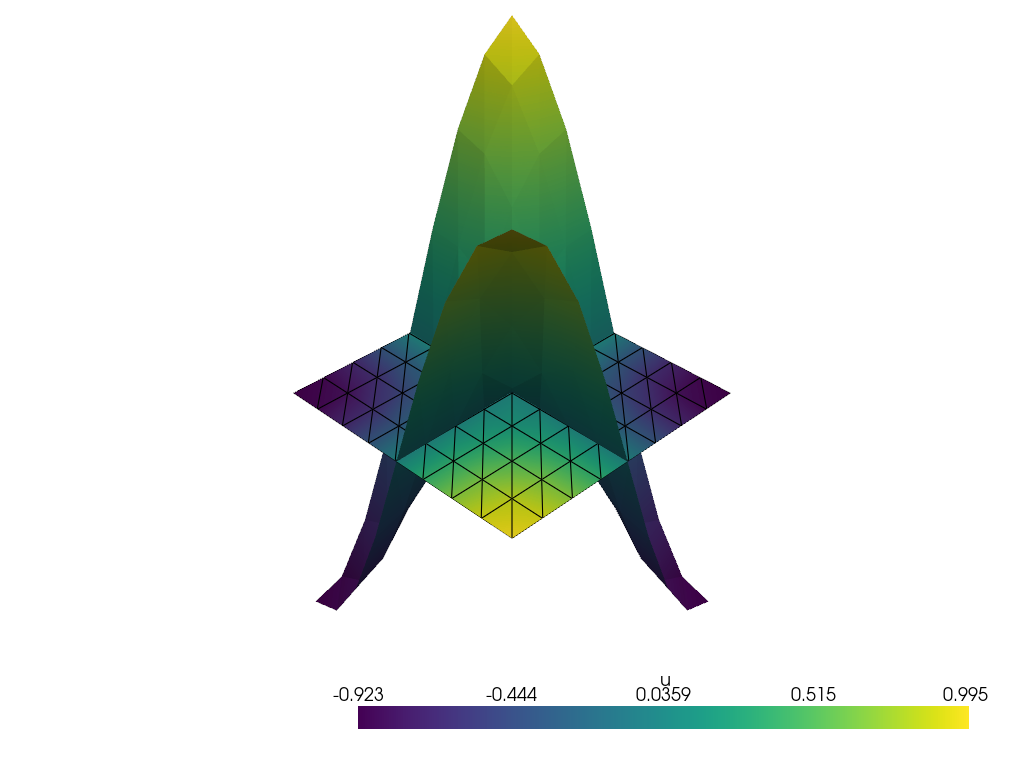
\includegraphics[width=\linewidth]{out_poisson/prob3_n8_d1_g-1.0.png}
        \caption{$P^1$, $2(8^2)$ cells}
    \end{subfigure}
    \begin{subfigure}{0.45\linewidth}
        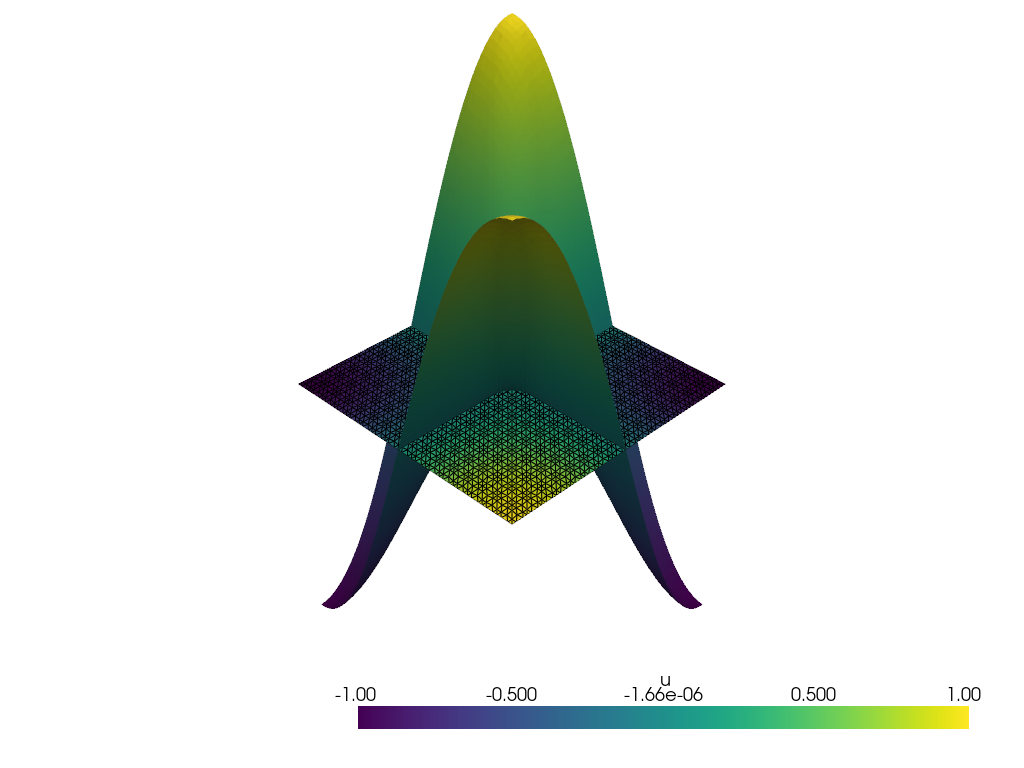
\includegraphics[width=\linewidth]{out_poisson/prob3_n16_d3_g-1.0.png}
        \caption{$P^3$, $2(16^2)$ cells}
    \end{subfigure}

    \caption{2D Poisson Results}\label{fig:p2-results}
\end{figure}

\begin{table}[h]
    \caption{2D Poisson Results}\label{tab:p2-results}

    \centering
    \begin{tabular}{c|c|c}
        $N_x, P^1$ & L2 error & Max. pointwise error\\
        4&    1.039e-01 & 2.538e-01\\
        8&    2.989e-02 & 8.766e-02\\
        16&   7.796e-03 & 2.649e-02\\
        32  & 1.972e-03 & 7.555e-03
    \end{tabular}
    \begin{tabular}{c|c|c}
        $N_x, P^3$ & L2 error & Max. pointwise error\\
        4&    3.189e-04 & 1.193e-03\\
        8&    1.946e-05 & 8.442e-05\\
        16&   1.199e-06 & 5.489e-06\\
        32  & 7.449e-08 & 3.459e-07 
    \end{tabular}
\end{table}

The solution converged with all values of 

\section{Biharmonic Problem}

\subsection{}

First, multiply the differential equation by $v \in \hz$ and integrate over $\Omega$,

\begin{equation}
    \intOm \left(\nabla^4 u\right)\, d\mu = \intOm fv \, d\mu,
\end{equation}

then apply Gauss Divergence Theorem,

\begin{equation}
    \cancelto{^{v(\Gamma) = 0 \,\forall v \in \hz}}{\int_{\Gamma} \left(\nabla^3 u \right) v dS }- \intOm \nabla^3 u \nabla v \, d\mu = \intOm fv \, d\mu,
\end{equation}

and applying Gauss Divergence Theorem once more,

\begin{equation}
    - \left[ \cancelto{^{\nabla v \cdot \hat{n}|_\Gamma = 0 \,\forall v \in \hz}}{\int_\Gamma \nabla^2 u (\nabla v \cdot \hat{n}) \, dS} - \intOm \nabla^2 u \nabla^2 v \, d\mu \right] = \intOm fv \, d\mu,
\end{equation}

which yields the weak form of the problem,

\begin{align}
    a(u, v) &= L(v) \quad \forall v \in \hz(\Omega)\\
    a(u, v)&=\intOm \nabla^2 u \nabla^2 v \, d\mu\\
    L(v) &= \intOm fv \, d\mu.
\end{align}

\subsection{}

As in the previous problems, $a(u, v)$ is symmetric by commutativity,

\begin{equation}
    a(u, v) = \intOm \nabla^2 u \nabla^2 v \, d\mu = \intOm \nabla^2 v \nabla^2 u \, d\mu = a(v, u).
\end{equation}

To show that $a(u, v)$ is continuous, first note that

\begin{equation}
    \norm{u}_\hz^2 = \norm{u}_\ltwo^2 + \norm{\nabla u}_\ltwo^2 + \norm{\nabla^2 u}_\ltwo^2,
\end{equation}

so

\begin{equation}
    \norm{\nabla^2 u}_\ltwo \leq \norm{u}_\hz.\label{eq:p4-inequality}
\end{equation}

and 

\begin{equation}
    \norm{ u}_\ltwo \leq \norm{u}_\hz.\label{eq:p4-inequality2}
\end{equation}

By the CS inequality,

\begin{equation}
    a(u, v) = \ip{\nabla^2 u}{\nabla^2 v}_\ltwo \leq \norm{\nabla^2 u}_\ltwo \norm{\nabla^2 v}_\ltwo.
\end{equation}

Using \autoref{eq:p4-inequality}, 

\begin{equation}
    \ip{\nabla^2 u}{\nabla^2 v}_\ltwo \leq \norm{u}_\hz \norm{v}_\hz
\end{equation}

and thus $a(u,v)$ is continuous. For $L(z)$, use the CS inequality,

\begin{equation}
    L(z) = \ip{f}{v}_\ltwo \leq \norm{f}_\ltwo \norm{v}_\ltwo
\end{equation}

and apply \autoref{eq:p4-inequality2},

\begin{equation}
    \ip{f}{v}_\ltwo \leq \norm{f}_\ltwo \norm{v}_\hz
\end{equation}

and thus $L(v)$ is continuous.

\subsection{}

\textbf{AI usage statement:} I provided Gemini with my code from Problem 3, and prompted it with the mixed formulation weak form shown below, then promted it to modify the Problem 3 code to solve the problem with mixed formulation.

The idea of the mixed formulation is to define some intermediate function $w$, such the fourth-order PDE becomes a system of two second-order PDEs,

\begin{align}
    -\nabla^2 w &= f\\
    -\nabla^2 u &= w
\end{align}
\begin{equation}
    u = \nabla u \cdot \hat{n} = 0\quad {\rm on} \Gamma.
\end{equation}

This formulation allows for enforcement of the boundary conditions through the bilinear form.

Using the mixed formualtion, some results are displayed in \autoref{fig:p4-results}, with some errors shown in \autoref{tab:p4-results}. Here, each increasing the degree of the test and trial functions led to about an order of magnitude of improvement in $L_2$ error. Additionally, using higher-degree polynomials leads to faster convergence with mesh refinement.


\begin{figure}[h]
    \centering
    \begin{subfigure}{0.45\linewidth}
        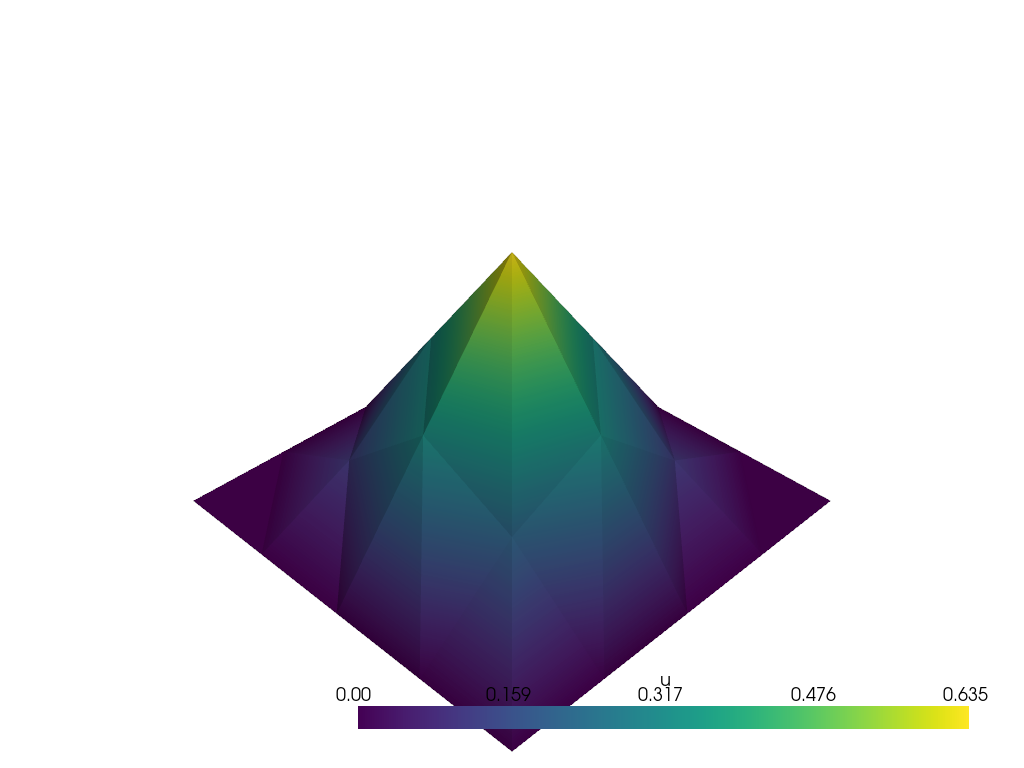
\includegraphics[width=\linewidth]{p4/prob4_n4_d1.png}
        \caption{$P^1$, $2(4^2)$ cells}
    \end{subfigure}
    \begin{subfigure}{0.45\linewidth}
        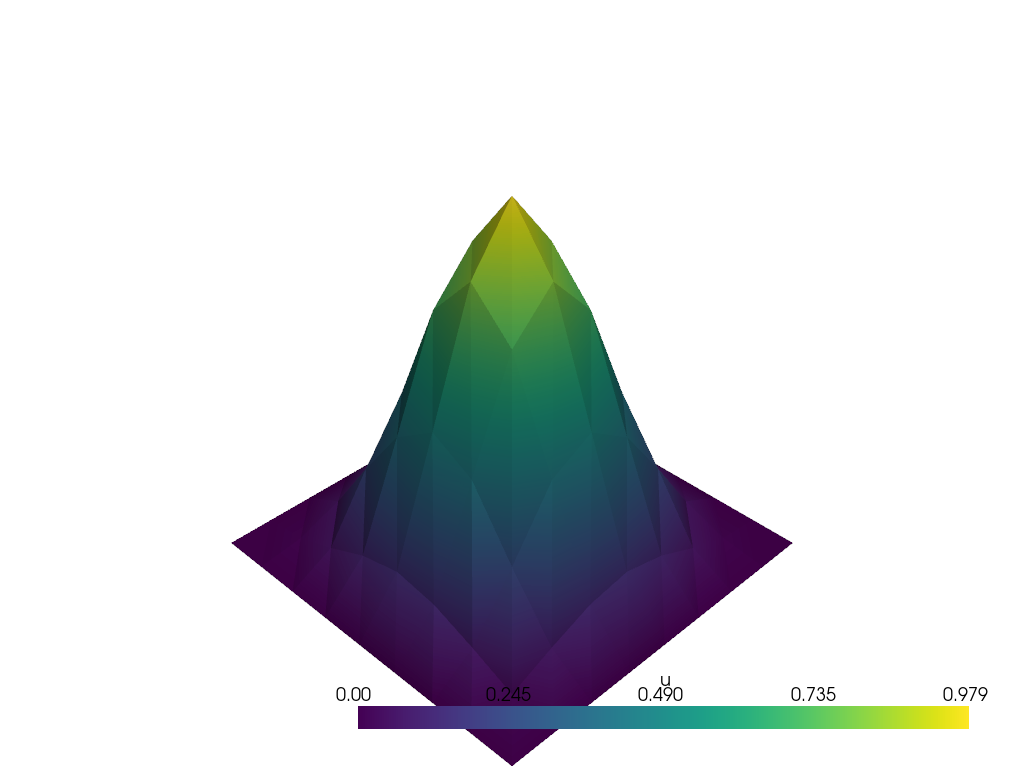
\includegraphics[width=\linewidth]{p4/prob4_n4_d2.png}
        \caption{$P^2$, $2(4^2)$ cells}
    \end{subfigure}

    \begin{subfigure}{0.45\linewidth}
        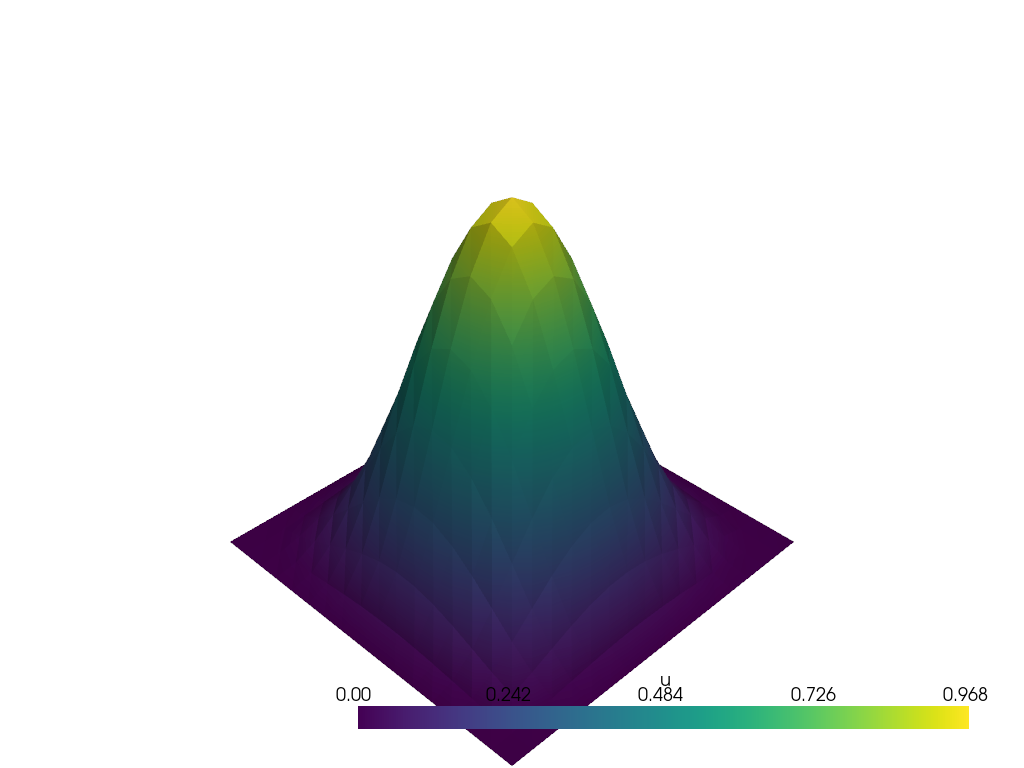
\includegraphics[width=\linewidth]{p4/prob4_n16_d1.png}
        \caption{$P^1$, $2(16^2)$ cells}
    \end{subfigure}

    \caption{2D Biharmonic Results}\label{fig:p4-results}
\end{figure}

\begin{table}[h]
    \caption{2D Biharmonic Results}\label{tab:p4-results}

    \centering
    \begin{tabular}{c|c|c}
        $N_x, P^1$ & L2 error & Max. pointwise error\\
        4&    1.701e-01 & 4.499e-01\\
        8&    5.774e-02 & 1.728e-01\\
        16&   1.575e-02 & 4.875e-02\\
        32  & 4.029e-03 & 1.273e-02
    \end{tabular}
    \begin{tabular}{c|c|c}
        $N_x, P^2$ & L2 error & Max. pointwise error\\
        4&    1.956e-02 & 6.008e-02\\
        8&    2.044e-03 & 6.797e-03\\
        16&   2.118e-04 & 7.854e-04\\
        32  & 2.410e-05 & 8.657e-05 
    \end{tabular}

    \begin{tabular}{c|c|c}
        $N_x, P^3$ & L2 error & Max. pointwise error\\
        4&    1.746e-03& 6.694e-03\\
        8&    9.373e-05& 3.736e-04\\
        16&   5.396e-06& 2.203e-05\\
        32  & 3.261e-07& 1.353e-06 
    \end{tabular}
\end{table}

\end{document}